\cleardoublepage
\section{Motivation}

\begin{figure}[!htbp]
    \label{fig:ideal_congestion_control}
    \begin{center}
        \leavevmode
        \ifpdf
        \resizebox{90mm}{!}{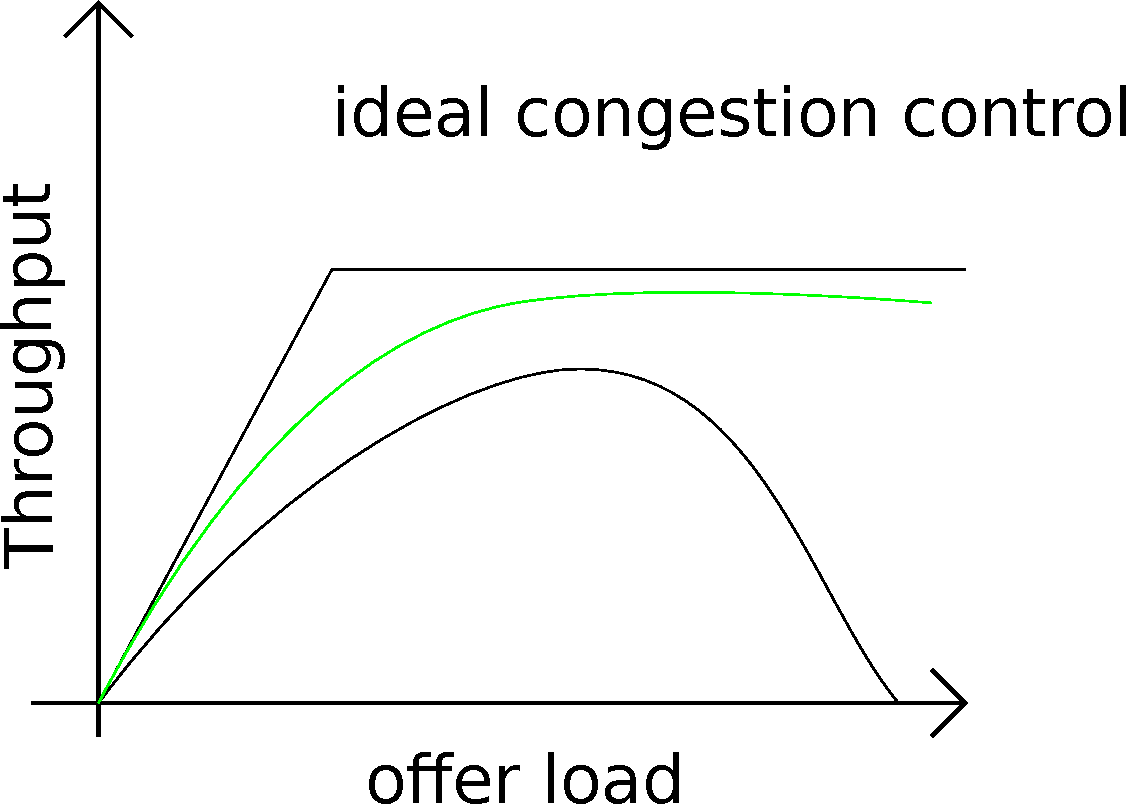
\includegraphics[height=6in]{ideal_congestion_control}}
        \else
        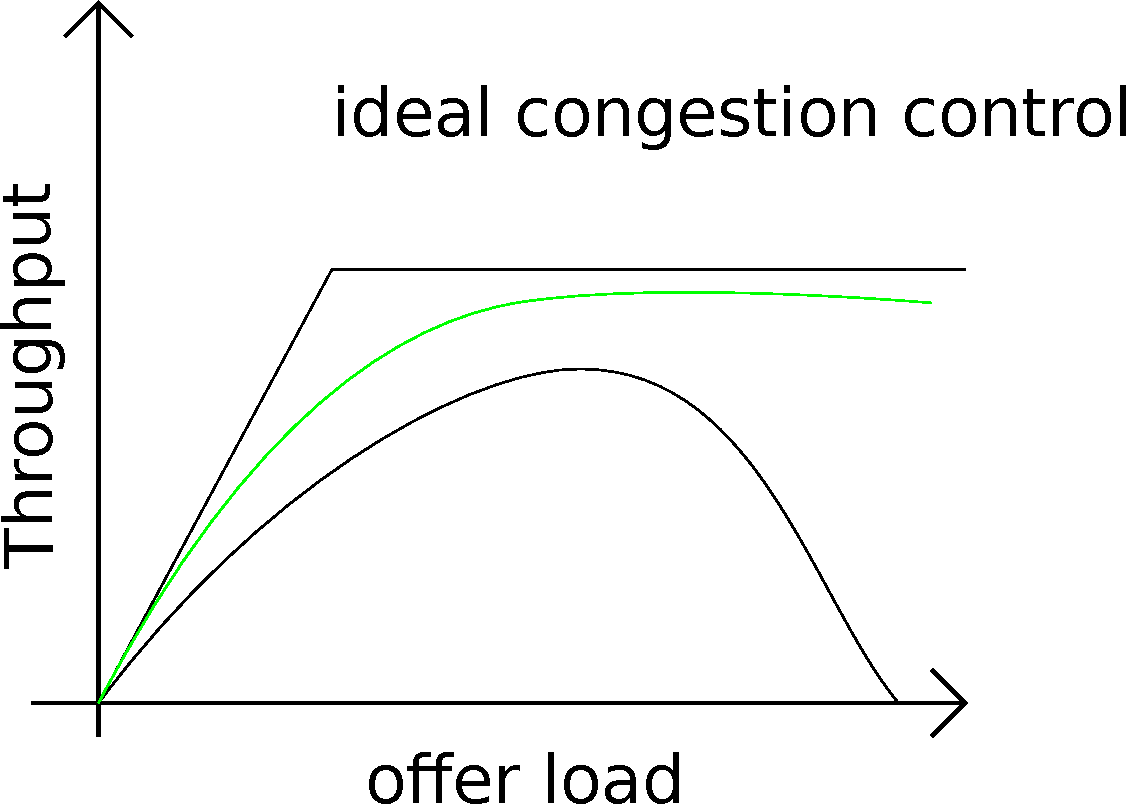
\includegraphics[bb = 92 86 545 742, height=6in]{ideal_congestion_control}
        \fi
        \caption{Congestion Control}
    \end{center}
\end{figure}

As figure \ref{fig:ideal_congestion_control} shows, The performance of network would reduce to zero if without any control. The ideal congestion control will enhance the network stability, and gain the capacity of network. However, in real network, the reaction delay much be token account. It only be closed to the ideal line. The green line show the real world congestion control. It may jitter since control packet loss or expired. In this study, I will develop a congestion control to
improve the throughput of network and reduce burst blocked probability.

There are several goals that congestion mechanism should achieve, the cost of implementation and deploy is cheap. That is said minimize additional hardware requirement and limited by router ability. Be fair among to all user.   

Congestion control is a comprehensive problem. The effective is very limited by control with any single method. Monitor and rate controller should co-operate to expand the effective. It may work with other mechanism, something like early drop packet, soft contention strategy.  
